\chapter{Opis problema}
\label{ch:opis-problema}
Ovaj rad bavi se problemom raspoznavanja studentskih identifikacijskih brojeva, poznatih pod skraćenicom
\emph{JMBAG}\footnote{\emph{Jedinstveni Matični Broj Akademskog Građana.}}. Ti se brojevi sastoje od deset znamenaka i
svakom studentu je dodijeljen jedinstveni broj koji služi kao identifikator studenta u sustavu hrvatskih fakulteta.
Kod pristupanja ispitima, od studenata se očekuje da uz ime i prezime također napišu svoj \emph{JMBAG} kako bi ih se
moglo jedinstveno identificirati u sustavu. Stoga je korisno napraviti sustav koji će moći automatski raspoznavati te
brojeve. Problem raspoznavanja \emph{JMBAG}-ova može se podijeliti u tri faze: pretprocesiranje, segmentacija i
klasifikacija. Faza pretprocesiranja služi kako bi se ulazna slika normalizirala te kako bi se znamenke odvojile od
pozadine. U fazi segmentacije potrebno je odrediti granice između pojedinačnih znamenki \emph{JMBAG}-a kako bi se svaka
znamenka mogla pojedinačno raspoznavati. Moguće je raspoznavati i više znamenki odjednom, ali tada klasifikator mora
biti kompleksniji i skup podataka za učenje mora biti veći. Zbog toga je poželjnije raspoznavati pojedinačne znamenke,
jer se skup za učenje efektivno poveća deset puta i sam klasifikator može biti jednostavniji. Posljednja faza
klasifikacije raspoznaje svaku znamenku pojedinačno. Slijednim spajanjem pojedinačno klasificiranih brojeva dobiva se
konačno raspoznati \emph{JMBAG}. U sljedećim odjeljcima bit će opisana implementacija navedenih faza raspoznavanja te
njihovo povezivanje u sustav za raspoznavanje \emph{JMBAG}-ova. Također će biti opisan način povezivanja navedenih faza
u konačan program kojim se trenira neuronska mreža te koji omogućuje raspoznavanje brojeva proizvoljnog broja znamenaka.


\section{Pretprocesiranje}
\label{sec:pretprocesiranje}
\begin{figure}[htb]
    \centering
    
\includegraphics[width=12cm]{images/preprocessing-original-image.png}
    \caption{\emph{JMBAG} prije pretprocesiranja.}
    \label{fig:preprocessing-original-image}
\end{figure}
Faza pretprocesiranja omogućuje jednoliko tretiranje ulaznih slika u preostalim fazama raspoznavanja. To se postiže na
način da se ulazna slika binarizira - dio slike koji predstavlja broj mora biti jasno odvojen od pozadine slike. Nakon
učitavanja slike u memoriju, prvi korak prema binarizaciji je uklanjanje svih boja iz slike. Time će se dobiti slika u
nijansama sive boje nad kojom se dalje može provesti postupak binarizacije. Kako bi se uklonila boja iz slike, za svaki
piksel računa se njegov intenzitet na sljedeći način:\\
\begin{equation*}
    I = \left(\frac{I_{crvena} + I_{zelena} + I_{plava}}{765}\right)^{2} \cdot 255.
\end{equation*}\\
Kako se piksel sastoji od komponenata $I_{crvena}$, $I_{zelena}$ i $I_{plava}$ čiji je raspon vrijednosti $[0, 255]$,
pri izračunu intenziteta njihov zbroj dijelimo sa zbrojem njihovih maksimalnih vrijednosti ($3 \cdot 255 = 765$).
Dobiveni rezultat zatim kvadriramo kako bi se bolje aproksimirala percepcija ljudskog oka na svjetlinu. Na kraju,
kvadrirani rezultat pomnoži se s $255$ kako bi se opet dobila vrijednost u rasponu $[0, 255]$. Dobiveni intenzitet $I$
zatim se koristi kao nova vrijednost komponenata $I_{crvena}$, $I_{zelena}$ i $I_{plava}$ za taj piksel.\\
\begin{figure}[htb]
    \centering
    
\includegraphics[width=12cm]{images/preprocessing-grayscale-image.png}
    \caption{\emph{JMBAG} nakon uklanjanja boje iz slike.}
    \label{fig:preprocessing-grayscale-image}
\end{figure}
Sada kada je za svaki piksel izračunat njegov intenzitet, može se provesti postupak binarizacije. Prvo je potrebno
pronaći minimalnu vrijednost intenziteta $I_{\min}$ i maksimalnu vrijednost intenziteta $I_{\max}$ na cijeloj slici za
sve potpuno vidljive piksele\footnote{Piksel se smatra potpuno vidljivim ako je vrijednost njegove neprozirnosti
jednaka $255$.}. Preko $I_{\min}$ i $I_{\max}$ računa se intenzitet odsijecanja:\\
\begin{equation*}
    I_{o} = \frac{I_{\max} - I_{\min}}{2}.
\end{equation*}\\
Intenzitet odsijecanja $I_{o}$ zatim se koristi kako bi se slika binarizirala na sljedeći način:
\begin{enumerate}
    \item Ako je vrijednost neprozirnosti piksela $(x, y)$ manja od $255$, piksel će pripadati pozadini.
    \item Ako je intenzitet piksela $(x, y)$ veći od intenziteta odsijecanja $I_{o}$, piksel će pripadati pozadini.
    \item Inače će piksel pripadati \emph{JMBAG}-u koji se raspoznaje.
\end{enumerate}
Kod binarizacije su pikseli pozadine bijele boje, dok su pikseli \emph{JMBAG}-a crne boje.
Slike\ \ref{fig:preprocessing-original-image},\ \ref{fig:preprocessing-grayscale-image}
i\ \ref{fig:preprocessing-binarized-image} prikazuju jedan \emph{JMBAG} kroz opisane korake pretprocesiranja.
\begin{figure}[htb]
    \centering
    
\includegraphics[width=12cm]{images/preprocessing-binarized-image.png}
    \caption{\emph{JMBAG} nakon postupka binarizacije.}
    \label{fig:preprocessing-binarized-image}
\end{figure}


\section{Segmentacija}
\label{sec:segmentacija}
Nakon binarizacije potrebno je pronaći granice među brojevima \emph{JMBAG}-a kako bi se oni mogli zasebno raspoznavati
u klasifikatoru. Kako slika dobivena postupkom binarizacije sadrži samo crnu i bijelu boju, za postupak segmentacije
korištena je pretpostavka da su brojevi na slici pojedinačno odvojene komponente. Stoga prvi korak segmentacije
pronalazi sve crne povezane komponente na slici te ih grupira u međusobno disjunktne skupove piksela koje će se u
daljnjem tekstu nazivati grupama piksela. U idealnom slučaju, svaka znamenka sastojat će se od samo jedne grupe piksela
koja je odvojena od svih ostalih grupa znamenaka, time ukupno tvoreći 10 grupa piksela. Ovakav slučaj prikazan je na
slici\ \ref{fig:ideal-segmentation} gdje je svaka grupa piksela obojena različitom bojom.
\begin{figure}[htb]
    \centering
    
\includegraphics[width=12cm]{images/ideal-segmentation.png}
    \caption{Idealno odvojene znamenke \emph{JMBAG}-a.}
    \label{fig:ideal-segmentation}
\end{figure}
Međutim, ovo neće uvijek biti slučaj te će neke slike sadržavati veći ili manji broj grupa piksela koje ne moraju nužno
odgovarati pojedinačnim znamenkama. Kako bi se za takve slike proveo postupak segmentacije, pronađene grupe piksela
dijele se na glavne grupe piksela i sporedne grupe piksela. Glavne grupe piksela čini skupina od najviše 10 grupa
piksela sa slike koje pojedinačno sadrže barem $\frac{1}{30}$ ukupnog broja crnih piksela na slici, dok su sve ostale
grupe sporedne grupe. Time je osigurano da će glavnih grupa uvijek biti 10 ili manje. Ovisno o broju pronađenih glavnih
grupa, implementirani algoritam segmentacije podešava skup glavnih grupa na sljedeći način:
\begin{enumerate}
    \item Ako je pronađeno 10 glavnih grupa, skup glavnih grupa ne treba podešavati.
    \item Ako je pronađeno 9 glavnih grupa, glavna grupa najveće širine uklanja se iz skupa glavnih grupa te se dijeli
    na pola po širini. Time se dobivaju dvije nove grupe piksela koje se dodaju u skup glavnih grupa koji tada sadrži
    ukupno 10 grupa.
    \item Ako je pronađeno 8 glavnih grupa, dvije glavne grupe najveće širine uklanjaju se iz skupa glavnih grupa.
    Zatim se uspoređuje omjer širina najšire i druge najšire uklonjene grupe. Ako je taj omjer veći ili jednak $1.33$,
    najšira grupa dijeli se na tri jednaka dijela po širini te se tako dobivene grupe uz preostalu grupu dodaju u skup
    glavnih grupa. S druge strane, ako je omjer širina manji od $1.33$ obje uklonjene grupe dijele se na pola po širini
    te se novonastale grupe dodaju u skup glavnih grupa. U oba slučaja, skup glavnih grupa sadržavat će ukupno 10 grupa.
    \item Ako je pronađeno 7 ili manje glavnih grupa, tada se $10 - n$ najširih grupa dijeli na pola po širini, gdje je
    $n$ broj pronađenih glavnih grupa.
\end{enumerate}
Ako nakon prethodnog koraka podešavanja skup glavnih grupa ne sadrži ukupno 10 grupa, algoritam segmentacije označava
sliku kao neispravnu te se postupak klasifikacije neće provoditi za tu sliku. U suprotnom, algoritam nastavlja s radom.
Slika\ \ref{fig:segmentation-division} prikazuje navedeni proces podešavanja glavnih grupa za slučaj 9 pronađenih glavnih
grupa. Stanje prije podešavanja glavnih grupa prikazuje najširu grupu označenu sivom bojom, dok su nakon postupka
podešavanja sve znamenke označene različitim bojama.\\
\begin{figure}[htb]
    \centering
    
\includegraphics[width=12cm]{images/segmentation-before-division.png}
    
\includegraphics[width=12cm]{images/segmentation-after-division.png}
    \caption{\emph{JMBAG} s dvije povezane znamenke prije i nakon podešavanja glavnih grupa piksela.}
    \label{fig:segmentation-division}
\end{figure}
Sljedeći korak jest pronaći kojim glavnim grupama teže pojedinačne sporedne grupe. Prvo se za svaku glavnu i sporednu
grupu računa središte $(x_s, y_s)$:\\
\begin{align*}
    x_s = \frac{\sum_{n = 1}^{N} x_n}{N}\\
    y_s = \frac{\sum_{n = 1}^{N} y_n}{N}
\end{align*}\\
gdje je $N$ broj crnih piksela u grupi. Za svako središte glavne grupe $(x_{s_g}, y_{s_g})$ i središte sporedne grupe
$(x_{s_s}, y_{s_s})$ računa se njihova međusobna \emph{Euklidska} udaljenost:\\
\begin{equation*}
    D = \sqrt{(x_{s_g} - x_{s_s})^{2} + (y_{s_g} - y_{s_s})^{2}}
\end{equation*}\\
te se svaka sporedna grupa pridjeljuje najbližoj glavnoj grupi. Nakon opisanog postupka postojat će 10 grupa piksela
na temelju kojih se svaka znamenka izdvaja u zasebnu sliku. Slika\ \ref{fig:assigned-minor-groups} prikazuje stanje
prije i nakon dodjeljivanja sporednih grupa (označenih crnom bojom) glavnim grupama.
\begin{figure}[htb]
    \centering
    
\includegraphics[width=12cm]{images/unassigned-minor-groups.png}
    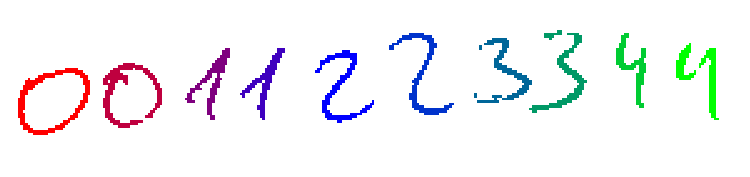
\includegraphics[width=12cm]{images/assigned-minor-groups.png}
    \caption{Glavne i sporedne grupe piksela prije i nakon postupka dodjeljivanja.}
    \label{fig:assigned-minor-groups}
\end{figure}


\section{Klasifikacija}
\label{sec:klasifikacija}
Postupkom segmentacije binarizirana slika podijeljena je na pojedinačne slike od kojih svaka sadrži jednu znamenku. Kao
klasifikator korištena je unaprijedna neuronska mreža s fiksnim brojem ulaza i izlaza, pa je stoga potrebno ulazne slike
svesti na određen broj značajki. Primjer segmentiranih znamenaka prikazan je na slici\ \ref{fig:segmented}. Segmentirane
slike su različitih dimenzija te njihov omjer visine i širine nije uvijek $1:1$.
\begin{figure}[htb]
    \centering
    \frame{
\includegraphics[width=1cm]{images/segmented-1.png}}
    \frame{
\includegraphics[width=1cm]{images/segmented-2.png}}
    \frame{
\includegraphics[width=1cm]{images/segmented-3.png}}
    \frame{
\includegraphics[width=1cm]{images/segmented-4.png}}
    \frame{
\includegraphics[width=1cm]{images/segmented-5.png}}
    \frame{
\includegraphics[width=1cm]{images/segmented-6.png}}
    \frame{
\includegraphics[width=1cm]{images/segmented-7.png}}
    \frame{
\includegraphics[width=1cm]{images/segmented-8.png}}
    \frame{
\includegraphics[width=1cm]{images/segmented-9.png}}
    \frame{
\includegraphics[width=1cm]{images/segmented-0.png}}
    \caption{Pojedinačne slike znamenaka nakon segmentiranja.}
    \label{fig:segmented}
\end{figure}
Također se crni pikseli nalaze na samom rubu svake slike. Stoga se segmentirane slike nadopunjavaju na način:
\begin{enumerate}
    \item Ako je visina slike veća od njene širine, slici se s lijeve i desne strane dodaju stupci bijelih piksela sve
    dok širina i visine nisu jednake.
    \item Ako je visina slike manja od njene širine, slici se s gornje i donje strane dodaju redovi bijelih piksela
    sve dok širina i visina slike nisu jednake.
\end{enumerate}
Nakon nadopunjavanja slika će uvijek imati omjer širine i visine jednak $1:1$, kao što je prikazano na
slici\ \ref{fig:scaled}.
\begin{figure}[htb]
    \centering
    \frame{
\includegraphics[width=1cm]{images/scaled-1.png}}
    \frame{
\includegraphics[width=1cm]{images/scaled-2.png}}
    \frame{
\includegraphics[width=1cm]{images/scaled-3.png}}
    \frame{
\includegraphics[width=1cm]{images/scaled-4.png}}
    \frame{
\includegraphics[width=1cm]{images/scaled-5.png}}
    \frame{
\includegraphics[width=1cm]{images/scaled-6.png}}
    \frame{
\includegraphics[width=1cm]{images/scaled-7.png}}
    \frame{
\includegraphics[width=1cm]{images/scaled-8.png}}
    \frame{
\includegraphics[width=1cm]{images/scaled-9.png}}
    \frame{
\includegraphics[width=1cm]{images/scaled-0.png}}
    \caption{Pojedinačne znamenke nakon ujednačavanja visine i širine.}
    \label{fig:scaled}
\end{figure}
Takva slika nadopunjava se još jednom sa svake strane tako da se dodaje obrub bijelih piksela. Obrub će povećati visinu
i širinu slike sa svake strane za $20\%$, tako de će se ukupna visina i širina slike povećati za $40\%$ što je prikazano
na slici\ \ref{fig:padding}.
\begin{figure}[htb]
    \centering
    \frame{
\includegraphics[width=1cm]{images/padding-1.png}}
    \frame{
\includegraphics[width=1cm]{images/padding-2.png}}
    \frame{
\includegraphics[width=1cm]{images/padding-3.png}}
    \frame{
\includegraphics[width=1cm]{images/padding-4.png}}
    \frame{
\includegraphics[width=1cm]{images/padding-5.png}}
    \frame{
\includegraphics[width=1cm]{images/padding-6.png}}
    \frame{
\includegraphics[width=1cm]{images/padding-7.png}}
    \frame{
\includegraphics[width=1cm]{images/padding-8.png}}
    \frame{
\includegraphics[width=1cm]{images/padding-9.png}}
    \frame{
\includegraphics[width=1cm]{images/padding-0.png}}
    \caption{Segmentiranje znamenke nakon konačnog postupka nadopunjavanja.}
    \label{fig:padding}
\end{figure}
Dimenzije slika nakon konačnog postupka nadopunjavanja i dalje nisu jednake za sve slike, te se stoga značajke odabiru
tako da se računaju udaljenosti do prvog crnog piksela počevši od nekog ruba slike. Također se računaju udaljenosti do
prvog crnog piksela počevši od središta slike. Ove udaljenosti prikazane su na
slici\ \ref{fig:features-for-single-digit} za jednu znamenku te na slici\ \ref{fig:features-for-multiple-digits} za svih
10 znamenaka. Na obje slike udaljenosti su označene različitim bojama na sljedeći način:
\begin{enumerate}
    \item Udaljenosti od vrha i dna slike za 4 jednoliko udaljena stupca označene su crvenom bojom.
    \item Udaljenosti s lijeve i desne strane slike za 4 jednoliko udaljena retka označene su plavom bojom.
    \item Dijagonalne udaljenosti sa sva 4 ruba slike označene su ljubičastom bojom.
    \item Udaljenosti od središta slike prema gore, dolje, lijevo i desno označene su zelenom bojom.
\end{enumerate}
\begin{figure}[htb]
    \centering
    \frame{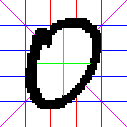
\includegraphics[width=5cm]{images/features-0.png}}
    \caption{Značajke za jednu znamenku \emph{JMBAG}-a.}
    \label{fig:features-for-single-digit}
\end{figure}
\begin{figure}[htb]
    \centering
    \frame{
\includegraphics[width=1cm]{images/features-1.png}}
    \frame{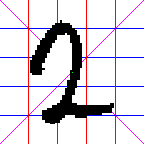
\includegraphics[width=1cm]{images/features-2.png}}
    \frame{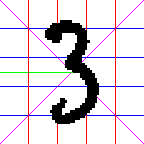
\includegraphics[width=1cm]{images/features-3.png}}
    \frame{
\includegraphics[width=1cm]{images/features-4.png}}
    \frame{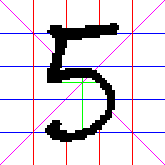
\includegraphics[width=1cm]{images/features-5.png}}
    \frame{
\includegraphics[width=1cm]{images/features-6.png}}
    \frame{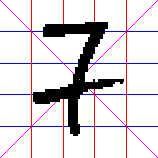
\includegraphics[width=1cm]{images/features-7.png}}
    \frame{
\includegraphics[width=1cm]{images/features-8.png}}
    \frame{
\includegraphics[width=1cm]{images/features-9.png}}
    \frame{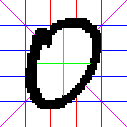
\includegraphics[width=1cm]{images/features-0.png}}
    \caption{Značajke za svih 10 znamenaka \emph{JMBAG}-a.}
    \label{fig:features-for-multiple-digits}
\end{figure}
Na ovaj način dobiveno je ukupno 24 udaljenosti koje se skaliraju na raspon $[0, 1]$ koristeći visinu i širinu slike.
Ovako skalirane udaljenosti koriste se kao značajke koje su ulaz unaprijedne neuronske mreže. Broj skrivenih slojeva
neuronske mreže nije fiksan te se može podešavati kod postupka učenja, što je opisano u sljedećem odjeljku. Neuronska
mreža ima ukupno 10 izlaza, jedan za svaku znamenku u rasponu $[0, 9]$. Vrijednosti svakog od izlaza su uvijek u rasponu
$[0, 1]$ te se stoga izlazi mreže mogu smatrati kao vjerojatnosti da ulazi predstavljaju svaku od znamenki. Kako bi se
odredila klasifikacije neke znamenke, uzima se vrijednost najvećeg izlaza mreže te se znamenka dodijeljena tom izlazu
uzima kao klasifikacija ulazne znamenke.


\section{Implementacija sustava za raspoznavanje}
\label{sec:implementacija-sustava-za-raspoznavanje}
